\documentclass[conference]{IEEEtran}
\IEEEoverridecommandlockouts
\usepackage{cite}
\usepackage{amsmath,amssymb,amsfonts}
\usepackage{algorithmic}
\usepackage{graphicx}
\usepackage{textcomp}
\usepackage{xcolor}
\usepackage{multirow}
\def\BibTeX{{\rm B\kern-.05em{\sc i\kern-.025em b}\kern-.08em
    T\kern-.1667em\lower.7ex\hbox{E}\kern-.125emX}}
\begin{document}

\title{Proactive Ensemble ML Autoscaling for Cloud-Native Microservices via Publish/Subscribe Event-Driven Architecture}

\author{
\IEEEauthorblockN{Ahmed El-Darawi}
\IEEEauthorblockA{\textit{Modern Science and Arts University}\\
Giza, Egypt \\
ahmed.eldarawii@gmail.com}
\and
\IEEEauthorblockN{Ahmed Ossama}
\IEEEauthorblockA{\textit{Modern Science and Arts University}\\
Giza, Egypt \\
ahmed.ossama1@gmail.com}
\and
\IEEEauthorblockN{Moamen Zaher}
\IEEEauthorblockA{\textit{LUT University}\\
Lappeenranta, Finland \\
moamen.zaher@lut.fi}
\and
\IEEEauthorblockN{Ammar Mohamed}
\IEEEauthorblockA{\textit{Cairo University}\\
Giza, Egypt \\
ammar@cu.edu.eg}
}

\maketitle

\begin{abstract}
Microservice architectures underpin modern cloud-native applications, yet their dynamic, highly multiplexed nature renders traditional reactive autoscaling approaches---such as the Kubernetes Horizontal Pod Autoscaler (HPA)---inadequate. Reactive systems detect workload changes only after performance degradation has occurred, leading either to Service-Level Agreement (SLA) violations or costly overprovisioning of compute resources. This paper presents a proactive ensemble ML autoscaling system that leverages asynchronous machine learning inference within a publish/subscribe event-driven architecture. A configurable ensemble of independently trained classifiers subscribes to per-service OS-level and application-level metrics, produces independent SLA-violation predictions, and forwards votes to a consensus service that applies majority-voting logic before issuing Kubernetes scaling commands. The architecture supports hot-swappable models, independent horizontal scaling of each component, and asymmetric scale-up/scale-down logic grounded in industry practice~\cite{lorido2014autoscaling}. The system is evaluated on the Sock Shop microservices benchmark~\cite{villamizar2017sockshop} using Locust-generated load profiles~\cite{locust}. Evaluation focuses on 95th-percentile tail latency, and resource utilisation relative to a baseline Kubernetes HPA deployment. This work advances sustainable cloud computing, contributing directly to SDG 12 (Responsible Consumption and Production) by minimising overprovisioning waste, and to SDG 9 (Industry, Innovation and Infrastructure) by introducing a novel, modular, production-ready scaling architecture.
\end{abstract}

\begin{IEEEkeywords}
proactive autoscaling, cloud-native microservices, ensemble machine learning, publish-subscribe architecture, Apache Kafka, Kubernetes HPA, SLA violation prediction, tail latency optimization, resource efficiency
\end{IEEEkeywords}

\section{Introduction}

Cloud-native microservice architectures promise elastic resource allocation as a first-class property, yet the dominant autoscaling mechanism in production Kubernetes clusters---the Horizontal Pod Autoscaler (HPA)---remains structurally reactive~\cite{hasan2020horizontal}. HPA monitors resource utilization metrics and scales deployments only after threshold violations occur. By the time CPU or memory thresholds are crossed, the application has already entered a degraded state. The remediation latency compounds the problem: Kubernetes must schedule new pods, pull container images, execute startup probes, and redistribute traffic through service meshes. During this window, which can span tens of seconds to minutes, user-facing latency degrades and SLA violations accumulate.

The reactive paradigm creates a fundamental tension. Conservative thresholds trigger scaling too late, causing SLA violations. Aggressive thresholds trigger scaling too early, wasting resources through overprovisioning. Neither strategy addresses the root cause: reaction is architecturally insufficient when the cost of remediation exceeds the detection window. Recent work in ML-based autoscaling~\cite{pbscaler,firm,autopilot} has demonstrated that proactive prediction can anticipate resource demands before degradation occurs, but existing systems either tightly couple prediction logic to specific frameworks, rely on single-model inference that amplifies false negative risk, or lack the architectural decoupling necessary for independent model evolution and horizontal scalability.

This paper presents a proactive autoscaling system that addresses these limitations through a fully decoupled publish/subscribe event-driven architecture. The system decouples metric aggregation, ML inference, and scaling decisions through Apache Kafka topics~\cite{garg2023kafka}, enabling independent horizontal scaling of each pipeline stage and hot-swappable model deployment without service interruption. An ensemble of three independently trained classifiers---Support Vector Machine (SVM)~\cite{svm}, Random Forest~\cite{randomforest}, and Logistic Regression~\cite{sklearn}---vote on scaling decisions through a consensus service, reducing false negative risk through diversity of inductive bias~\cite{ensemble}. The architecture implements asymmetric scale-up/scale-down logic grounded in industry practice: immediate scale-up on ML prediction, conservative scale-down only after sustained low resource utilization, mirroring the design philosophy documented in autoscaling literature~\cite{lorido2014autoscaling} and production systems~\cite{autopilot}. A feature engineering methodology prioritizes trajectory signals (delta features) over instantaneous metrics, grounded in the observation that a system at high CPU but stable load is less dangerous than a system at moderate CPU with accelerating demand. This approach achieves sub-10ms prediction latency through trend-based features computed from metric deltas rather than time-series models, enabling proactive scaling in latency-critical systems where LSTM or ARIMA approaches would introduce prohibitive overhead that exceeds pod startup windows~\cite{pbscaler}.

The system is evaluated on the Sock Shop microservices benchmark~\cite{villamizar2017sockshop}, a polyglot e-commerce application comprising seven independently scalable services (Figure~\ref{fig:sockshop}). Load is generated using Locust~\cite{locust} with ramp profiles that simulate organic traffic growth. Metrics are scraped from Prometheus~\cite{prometheus} at a 30-second polling interval derived from four converging constraints: the industry-standard Prometheus scrape interval range (15-60 seconds), the rate() function's Nyquist-analog requirement for accurate derivative computation, the pod startup lead time chain in Kubernetes, and the temporal sensitivity of delta features that encode trajectory rather than instantaneous state.

\begin{figure}[htbp]
\centerline{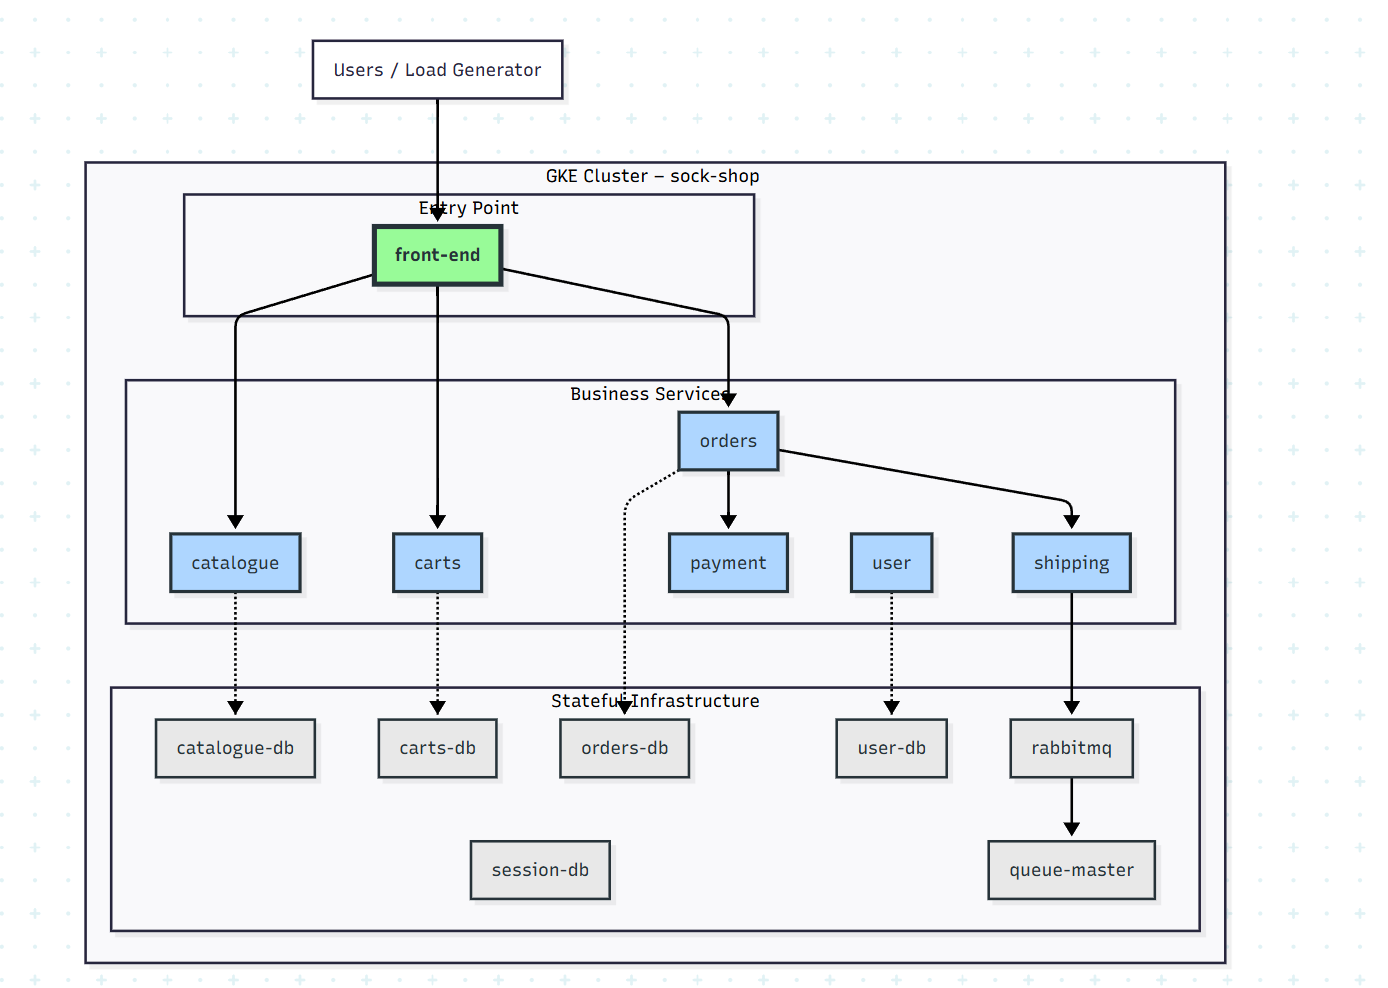
\includegraphics[width=0.9\columnwidth]{sockshop.png}}
\caption{Weaveworks Sock Shop microservices architecture.}
\label{fig:sockshop}
\end{figure}

\section{Background and Related Work}

\subsection{Reactive Autoscaling Baselines}

The Kubernetes Horizontal Pod Autoscaler (HPA) represents the production baseline for container autoscaling. HPA polls the Metrics Server at configurable intervals (default 15 seconds) and computes a desired replica count based on the ratio of current to target resource utilization. When the ratio exceeds a threshold, HPA issues a scale command to the Deployment controller. The mechanism is purely reactive: scaling occurs only after metrics cross thresholds, and the control loop has no predictive component. HPA's stabilization window (default 5 minutes for scale-down) prevents oscillation but further delays response to decreasing load.

Event-driven autoscaling systems extend HPA with triggers from external sources such as message queue depth or custom metrics. While these systems broaden the input signal space, they remain reactive: scaling decisions are threshold-based responses to current state rather than predictions of future state. Both HPA and KEDA share a fundamental limitation: by the time a threshold is crossed, the application has already entered a degraded state, and the remediation latency (pod scheduling, image pull, startup probes, traffic redistribution) extends the damage window.

\subsection{Proactive and ML-Based Autoscaling}

PBScaler addresses reactive limitations through proactive prediction~\cite{pbscaler}. PBScaler trains LSTM models on historical workload traces and predicts future resource demands at sub-minute granularity. The system demonstrates that proactive scaling can reduce SLA violations compared to reactive baselines, but PBScaler tightly couples prediction logic to a monolithic service and does not address the architectural requirements for independent model evolution or horizontal scalability of the inference pipeline.


FIRM (Fast In-memory Request-level Modeling)~\cite{firm} takes a different approach by modeling request-level resource consumption and predicting aggregate demand through simulation. FIRM achieves sub-second prediction latency by maintaining in-memory models of per-request resource profiles. The system demonstrates that fine-grained modeling can improve prediction accuracy, but FIRM requires instrumentation of application code to capture request-level traces, limiting its applicability to black-box microservices. Additionally, FIRM's single-model architecture does not provide the fault tolerance benefits of ensemble methods.

Autopilot~\cite{autopilot}, deployed in Google's Borg cluster manager, uses ML to predict resource usage and right-size container resource requests. Autopilot trains models on historical usage patterns and adjusts resource allocations to minimize slack while avoiding out-of-memory kills. While Autopilot demonstrates the value of ML-driven resource management at scale, it focuses on vertical scaling (resource request adjustment) rather than horizontal scaling (replica count adjustment), and its integration with Borg's proprietary infrastructure limits transferability to Kubernetes environments.

This system differs from existing approaches in three ways. First, it decouples metric aggregation, inference, and decision-making through Kafka topics, enabling independent horizontal scaling and hot-swappable model deployment. Second, it employs an ensemble of three classifiers with diverse inductive biases, reducing false negative risk through majority voting. Third, it implements asymmetric scale-up/scale-down logic that mirrors production practice documented in autoscaling literature~\cite{lorido2014autoscaling,autopilot}.

\subsection{Event-Driven Observability Pipelines}

Apache Kafka has emerged as the de facto standard for building event-driven data pipelines in cloud-native systems. Kafka's publish/subscribe model decouples producers from consumers through durable, partitioned topics. This architectural pattern enables independent scaling of pipeline stages: metric producers can scale independently of inference consumers, and inference consumers can scale independently of decision services. Kafka's consumer group abstraction provides automatic load balancing and fault tolerance, ensuring that message processing continues even if individual consumers fail.


In the context of ML-based autoscaling, Kafka provides three critical properties. First, Kafka decouples the metric aggregation service from inference services, allowing models to be retrained and redeployed without modifying the metric collection logic. Second, Kafka enables horizontal scaling of inference services: multiple instances of the same model can consume from the same topic partition, and different models can consume from different partitions, providing both intra-model and inter-model parallelism. Third, Kafka's durability guarantees ensure that votes are not lost during transient failures, enabling the consensus service to make decisions based on complete information even in the presence of network partitions or service restarts.

\subsection{Ensemble Classification in Operational Decision-Making}

Ensemble methods combine predictions from multiple models to produce a final decision that is more robust than any individual model. The theoretical foundation rests on the bias-variance decomposition: if individual models have uncorrelated errors, the ensemble's error is reduced by averaging. In the context of SLA violation prediction, ensemble methods provide a critical operational benefit: they reduce false negative risk. A false negative (missed SLA violation) has worse consequences than a false positive (unnecessary scale-up), because a missed violation directly impacts user experience while an unnecessary scale-up merely wastes resources temporarily.

The ensemble comprises three classifiers with diverse inductive biases. Support Vector Machine (SVM) employs gradient-boosted decision trees, which excel at learning complex feature interactions through sequential error correction. Random Forest uses bagging to reduce variance through bootstrap aggregation of independent trees. Logistic Regression provides a linear baseline with probabilistic calibration that tends toward high recall due to its decision boundary geometry. The diversity of these approaches ensures that the ensemble's failure modes are uncorrelated: a workload pattern that causes SVM to miss a violation may still be detected by Random Forest or Logistic Regression.


The gap that this work addresses is the absence of a system that combines proactive ensemble ML inference with a fully decoupled publish/subscribe architecture and asymmetric consensus-gated scaling logic. Existing ML-based autoscalers either employ single-model inference (amplifying false negative risk), tightly couple components (preventing independent evolution), or lack the asymmetric scale-up/scale-down logic necessary for production deployment. This system demonstrates that these properties can be achieved simultaneously through careful architectural design grounded in the operational requirements of cloud-native systems.

\section{System Architecture}

The architecture comprises five components connected through two Kafka topics~\cite{garg2023kafka}. The metrics aggregator service polls Prometheus~\cite{prometheus} at a fixed interval, constructs feature vectors from raw metrics, and publishes them to the \texttt{metrics} topic. Three ML inference services---Support Vector Machine (SVM)~\cite{svm}, Random Forest~\cite{randomforest}, and Logistic Regression~\cite{sklearn}---subscribe to the \texttt{metrics} topic, perform independent inference, and publish votes to the \texttt{model-votes} topic. The authoritative scaling service subscribes to the \texttt{model-votes} topic, aggregates votes using majority-voting logic, and outputs scaling decisions. In production mode, the scaling service can execute decisions by invoking the Kubernetes API~\cite{hasan2020horizontal}; in evaluation mode, decisions are logged for analysis. Figure~\ref{fig:sysarch} illustrates the complete system architecture.

\begin{figure}[htbp]
\centerline{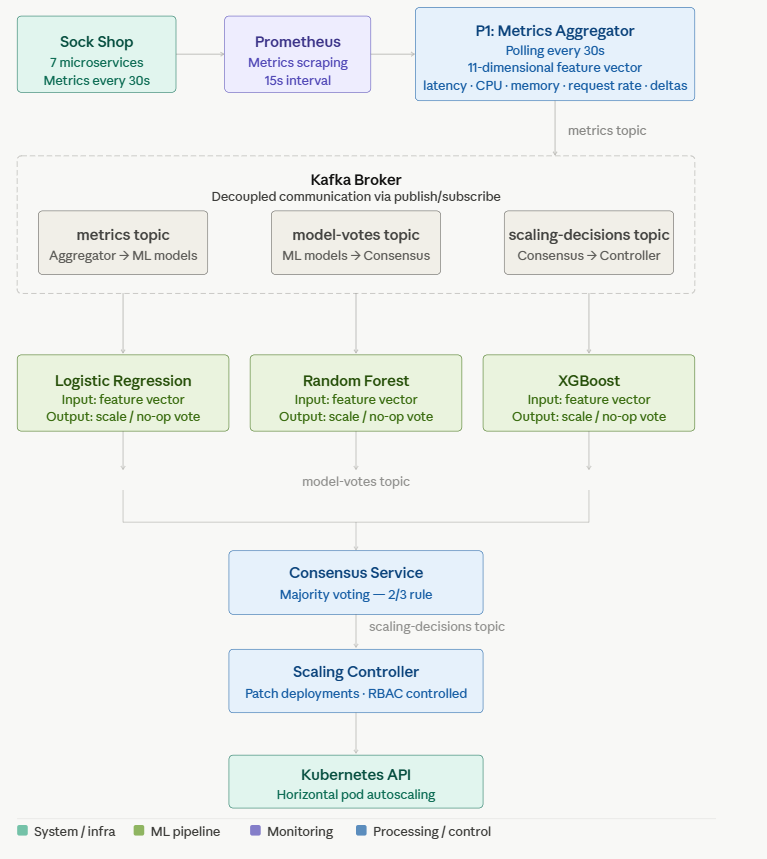
\includegraphics[width=\columnwidth]{sys-arch.png}}
\caption{System architecture showing the publish/subscribe event-driven pipeline.}
\label{fig:sysarch}
\end{figure}

\subsection{Metrics Aggregator Service}

The metrics aggregator service polls Prometheus every 30 seconds and constructs feature vectors for each monitored service. The polling interval is derived from four converging constraints. First, the industry-standard Prometheus scrape interval ranges from 15 to 60 seconds, establishing the lower bound on meaningful aggregation windows. Second, Prometheus's rate() function requires at least two samples per window to compute accurate derivatives, imposing a Nyquist-analog constraint on the polling frequency. Third, Kubernetes pod startup latency (image pull, container initialization, readiness probes) typically spans 30 to 90 seconds, defining the lead time required for proactive scaling to be effective. Fourth, delta features that encode trajectory (rate of change in CPU, latency, throughput) require sufficient temporal separation to capture meaningful trends without being dominated by measurement noise.


The chosen interval satisfies all four constraints simultaneously: it exceeds the minimum Prometheus scrape interval, provides sufficient samples for rate() computation, aligns with pod startup lead time, and captures trajectory signals without excessive noise. The aggregator queries Prometheus using PromQL expressions that compute per-service request rates, error rates, latency percentiles (p50, p95, p99), CPU utilization, and memory consumption. These raw metrics are combined with delta features computed from the previous polling window to form a 17-dimensional feature vector: 10 base metrics plus 7 one-hot encoded service features.

The aggregator operates in two modes. In production mode, feature vectors are published to the Kafka \texttt{metrics} topic for consumption by inference services. In development mode, feature vectors are written to CSV files for model retraining. This dual-mode design enables continuous improvement: production deployments generate labeled data (metrics paired with observed SLA violations), which can be used to retrain models offline without modifying the production pipeline. The mode is controlled by an environment variable, allowing the same container image to serve both purposes.

The aggregator maintains a stateful cache of previous metrics to compute delta features. When a service is first observed, delta features are initialized to zero. This design choice reflects the operational reality that trajectory signals are unavailable for newly deployed services, and the models must make predictions based solely on instantaneous metrics until sufficient history accumulates. The cache is implemented as an in-memory dictionary keyed by service name, with no persistence across restarts. This stateless-by-default design simplifies deployment and recovery: if the aggregator crashes, it resumes polling from the current state without requiring external state reconstruction.


\subsection{ML Inference Services}

Three inference services consume feature vectors from the \texttt{metrics} topic and publish votes to the \texttt{model-votes} topic. Each service is containerized with a pre-trained model loaded from a volume-mounted directory. The volume-mount design enables hot-swappable model deployment: a new model can be deployed by updating the volume contents and restarting the container, without rebuilding the container image or modifying the inference service code. This separation of model artifacts from service logic is critical for operational flexibility, as model retraining cycles are typically much faster than service deployment cycles.

Each inference service implements a shared preprocessing pipeline that mirrors the training-time transformations. Missing values and infinities are replaced with zero, matching the training-time imputation strategy. For Logistic Regression, features are standardized using a StandardScaler fitted during training and serialized alongside the model. XGBoost and Random Forest operate directly on raw features without scaling.

The inference service loads the model, parameters, and performance metrics from JSON files stored alongside the serialized model. The parameters file contains the service mapping and hyperparameters used during training, ensuring that inference-time preprocessing matches training-time preprocessing exactly. The metrics file contains test-set performance statistics (accuracy, precision, recall, ROC-AUC) that can be logged for monitoring and debugging. This metadata-rich model packaging enables the consensus service to weight votes based on model performance if desired, though the current implementation uses unweighted majority voting.


Each inference service publishes a vote message containing the service name, model name, binary prediction (0 for no action, 1 for scale up), probability of the predicted class, and confidence (maximum probability across classes). The vote message is serialized as JSON and published to the \texttt{model-votes} topic with the service name as the message key, ensuring that all votes for a given service are routed to the same Kafka partition. This partitioning strategy enables the consensus service to consume votes in service-order without requiring cross-partition coordination.

The inference services operate asynchronously and independently. Each service maintains its own Kafka consumer group, ensuring that messages are load-balanced across instances if multiple replicas are deployed. The services do not coordinate with each other: if one service crashes or falls behind, the other services continue processing. This isolation property is critical for fault tolerance: a bug in one model's inference logic cannot cascade to other models. The consensus service handles incomplete vote sets gracefully, making decisions based on available votes if the decision window expires before all models respond.

\subsection{Authoritative Scaling Service}

The authoritative scaling service subscribes to the \texttt{model-votes} topic and aggregates votes using a configurable voting strategy. The default strategy is majority voting: if two or more models vote for scale-up, the decision is scale-up; otherwise, the decision is no action. Alternative strategies include unanimous voting (all models must agree) and weighted voting (votes are weighted by model confidence). The voting strategy is controlled by an environment variable, enabling experimentation without code changes.


The consensus service implements a time-windowed aggregation strategy. When the first vote for a service arrives, a timer starts. If all three votes arrive before the window expires (default 5 seconds), the decision is made immediately. If the window expires with incomplete votes, the decision is made based on available votes. This design balances responsiveness with completeness: in the common case where all models respond quickly, decisions are made with full information; in the failure case where a model is slow or crashed, decisions are still made to avoid blocking the pipeline.

The consensus service maintains a vote buffer keyed by service name. When a decision is made, the buffer for that service is cleared and the decision is logged. The service outputs human-readable decision summaries showing which models voted for which action, the vote count, and the average confidence. This transparency is critical for operational debugging: when a scaling decision is questioned, operators can inspect the logs to understand which models contributed to the decision and with what confidence.

The consensus service implements asymmetric scale-up/scale-down logic grounded in production practice~\cite{lorido2014autoscaling}. Scale-up decisions are executed immediately when the majority vote indicates scale-up. Scale-down decisions are gated by a policy that requires sustained low resource utilization: CPU must remain below a threshold (default 30\%) for a sustained window (default 10 minutes) before scale-down is permitted. This asymmetry reflects the operational reality that scaling up too aggressively wastes resources temporarily, while scaling down too aggressively risks SLA violations that directly impact users. The policy mirrors established autoscaling practices that specify stabilization windows for scale-down to prevent oscillation~\cite{hasan2020horizontal}.


\subsection{Kafka Topics and Partitioning}

The system uses two Kafka topics to decouple pipeline stages. The \texttt{metrics} topic carries feature vectors from the aggregator to inference services. Messages are keyed by service name and contain a timestamp, service identifier, and 17-dimensional feature vector (10 base metrics plus 7 one-hot encoded service features). The topic is configured with a single partition to preserve message ordering, ensuring that inference services process metrics in temporal order. This ordering property simplifies stateful inference if models require temporal context, though the current models are stateless.

The \texttt{model-votes} topic carries votes from inference services to the consensus service. Messages are keyed by service name and contain the model name, prediction, probability, and confidence. The topic is configured with three partitions to enable parallel consumption by the consensus service if multiple instances are deployed. The service-name key ensures that all votes for a given service are routed to the same partition, enabling the consensus service to aggregate votes without cross-partition coordination.

Kafka's durability guarantees ensure that messages are not lost during transient failures. If an inference service crashes, it resumes consumption from its last committed offset, reprocessing any messages that were consumed but not acknowledged before the crash. If the consensus service crashes, it resumes from its last committed offset, ensuring that no votes are lost. This at-least-once delivery semantic is acceptable for autoscaling: duplicate votes are idempotent (the consensus service deduplicates based on message timestamp), and the cost of reprocessing is negligible compared to the cost of missing a vote.





\section{Feature Engineering and Label Construction}

\subsection{Feature Vector Design}

The feature vector comprises 17 dimensions organized into five groups: (1) throughput (request rate), (2) reliability (error rate), (3) latency percentiles (p50, p95, p99), (4) resource utilization (CPU percentage, memory MB), and (5) delta features (rate of change in request rate, p95 latency, and CPU utilization). Service identity is one-hot encoded into 7 binary features (service\_0 through service\_6), enabling models to learn service-specific patterns without imposing false ordinal relationships.

Delta features encode trajectory rather than instantaneous state. A system at high CPU but stable load is less dangerous than one at moderate CPU with rapidly accelerating demand. Delta features compute the difference between current and previous (30 seconds ago) metric values, capturing acceleration signals that predict violations before resource limits are reached. Request rate delta captures workload acceleration, p95 latency delta captures tail latency degradation, and CPU delta captures resource pressure acceleration.

\subsection{Label Construction}

The binary classification target is constructed using a lookahead window methodology. For each metric observation at time $t$, the label is 1 (violation) if any p95 latency measurement in the window $[t, t+60s]$ exceeds the SLA threshold, and 0 (no violation) otherwise. The 60-second lookahead window is chosen to match the pod startup latency: if a violation will occur within the next 60 seconds, the system should scale up now to ensure that new pods are ready before the violation occurs.

The SLA threshold is derived empirically using a percentile-based methodology grounded in the operational reality that no contractual SLA exists for the Sock Shop benchmark. The system is run under comfortable load (constant pattern, 50 users) to observe the p95 latency the front-end naturally produces under normal operating conditions. The P75 of these observations is taken as the SLA threshold, representing the upper bound of normal behavior: 25\% of comfortable-load observations exceed it, capturing the tail of normal variance without being so tight that routine fluctuations trigger violations. For the GKE deployment, this methodology yields a threshold of 35.68ms. Front-end p95 latency is chosen as the signal because front-end is the user-facing entry point that every request passes through, aggregating the effect of all downstream service degradation into a single observable metric.

This label construction produces a binary classification problem rather than a multiclass problem. The system predicts whether to scale up (1) or take no action (0). Scale-down is deliberately excluded from the ML classification scope and handled by the policy-based logic in the consensus service. This design choice is grounded in the observation that scale-down is fundamentally a temporal stability problem rather than a prediction problem. Kubernetes HPA's 5-minute stabilization window for scale-down reflects the same insight: scale-down should occur only after sustained low utilization, not based on instantaneous predictions. By separating scale-up prediction (ML-driven) from scale-down policy (rule-based), the system aligns with production practice and avoids the risk of ML-driven scale-down causing oscillation.


\subsection{Dataset Characteristics}

The training dataset comprises 3,570 samples collected from a 4-hour mixed pattern run on Google Kubernetes Engine (GKE). The GKE cluster consists of 3 nodes of type e2-standard-4 (4 vCPU, 16 GB RAM each) in region us-central1-a. Figure~\ref{fig:expsetup} illustrates the complete experimental setup including the GKE cluster, load generation, and monitoring infrastructure.

\begin{figure}[htbp]
\centerline{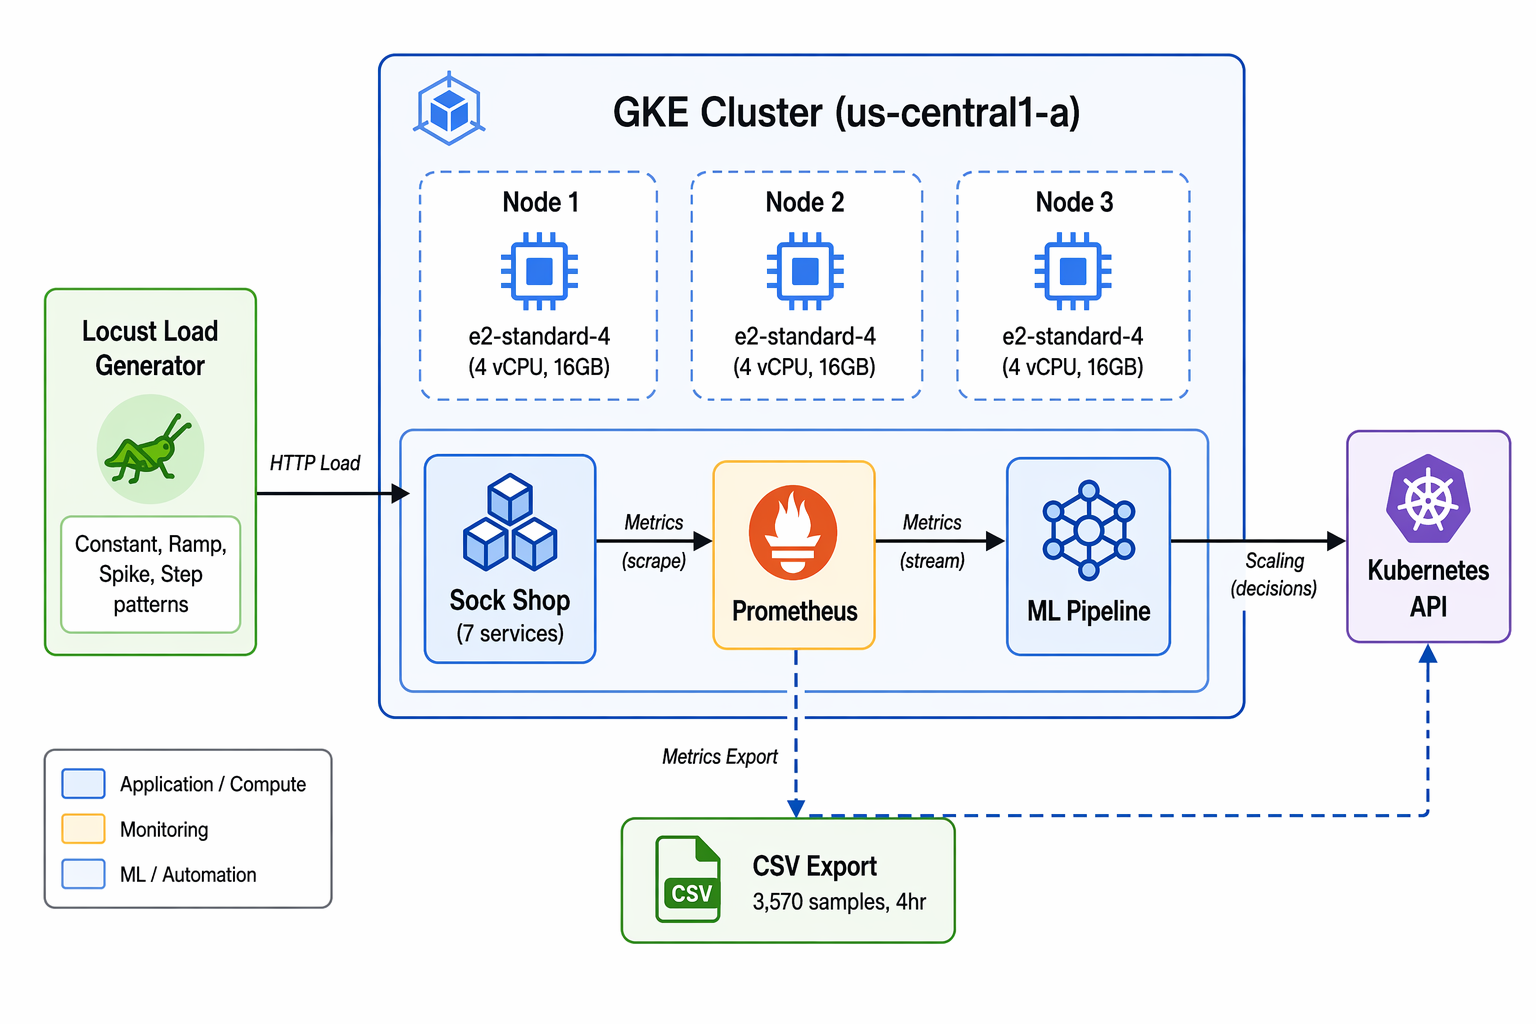
\includegraphics[width=\columnwidth]{experiment-setup.png}}
\caption{Experimental setup showing load generation, monitoring, and autoscaling components.}
\label{fig:expsetup}
\end{figure}

The dataset exhibits significant class imbalance: 13.3\% of samples are labeled as violations (475 positive samples, 3,095 negative samples). The imbalance reflects the operational reality that SLA violations are rare events under the derived threshold of 35.68ms. The dataset is split into training (80\%) and test (20\%) sets using stratified sampling to preserve class distribution.

The violation distribution is non-uniform across services and load patterns. The front-end, catalogue, and orders services account for the majority of violations, reflecting their position in the request path and their role as aggregation points for downstream service calls. The payment and shipping services exhibit fewer violations, as they are invoked less frequently and have simpler logic. The user and carts services exhibit the fewest violations, as they serve primarily read-heavy workloads with minimal computational overhead. Across patterns, step and ramp patterns produce the highest violation rates (88.6\% and 81.8\% of loaded rows exceeding threshold), while constant produces the lowest (24.6\%), validating that the threshold discriminates between stressed and comfortable load conditions. The one-hot encoded service features enable the models to learn these service-specific violation patterns while maintaining the ability to generalize across services through the shared base metrics.

SMOTE (Synthetic Minority Over-sampling Technique)~\cite{smote} is applied to the training set only to address class imbalance. SMOTE generates synthetic positive samples by interpolating between existing positive samples in feature space, producing a balanced training set with 50\% positive and 50\% negative samples (sampling\_strategy=1.0). Critically, SMOTE is not applied to the test set. Applying SMOTE to the test set would contaminate the evaluation by introducing synthetic samples that do not reflect real system behavior, artificially inflating performance metrics. This methodological integrity is essential for valid conclusions: the test set must represent the true distribution of violations in production, including the class imbalance, to provide unbiased performance estimates.


\section{Ensemble Design and Evaluation}

\subsection{Model Selection and Training}

The ensemble comprises three classifiers with diverse inductive biases: Support Vector Machine (SVM) with RBF kernel, Random Forest (bagged decision trees), and Logistic Regression (linear classifier). SVM employs non-linear decision boundaries through kernel transformations, excelling at capturing complex feature interactions in high-dimensional spaces. Random Forest uses bootstrap aggregation to reduce variance through independent tree ensembles. Logistic Regression provides a linear baseline with probabilistic calibration. The diversity of these approaches ensures that the ensemble's failure modes are uncorrelated: a workload pattern that causes one model to miss a violation may still be detected by others.

All models are trained on the GKE mixed dataset using a standard 80/20 stratified split. The training set (80\%, 2,856 samples) is balanced using SMOTE to achieve 50/50 class distribution. The test set (20\%, 714 samples) preserves the natural violation rate to provide unbiased performance estimates. The service identity feature is one-hot encoded into 7 binary features, resulting in a 17-dimensional feature vector comprising throughput, latency, resource, delta, and service features. This encoding enables models to learn service-specific violation patterns while preventing false ordinal relationships between services.

Hyperparameters are tuned using 5-fold cross-validation on the training set. SVM uses RBF kernel with balanced class weights and probability estimates enabled for ROC-AUC computation. Random Forest uses 200 estimators with max\_depth=8 and balanced class weights. Logistic Regression uses L2 regularization with balanced class weights and applies StandardScaler normalization. Models are serialized using joblib and packaged with preprocessing metadata to ensure inference-time consistency.

\subsection{Model Performance Results}

Table~\ref{tab:gke-results} presents test-set performance for all three models. Random Forest achieves the highest overall performance with 95.8\% recall and 99.3\% ROC-AUC, missing only 4 violations out of 95 in the test set. SVM achieves 98.9\% recall with 98.3\% ROC-AUC, missing only 1 violation. Logistic Regression achieves 99.0\% recall, missing only 1 violation, though with lower precision (66.0\%) reflecting its conservative decision boundary.

\begin{table}[htbp]
\caption{Model Performance}
\begin{center}
\begin{tabular}{|l|c|c|c|c|}
\hline
\textbf{Model} & \textbf{Precision(1)} & \textbf{Recall(1)} & \textbf{F1(1)} & \textbf{ROC-AUC} \\
\hline
SVM & 0.657 & 0.989 & 0.790 & 0.983 \\
Random Forest & 0.752 & 0.958 & 0.843 & 0.993 \\
Logistic Regression & 0.660 & 0.990 & 0.795 & 0.995 \\
\hline
\end{tabular}
\label{tab:gke-results}
\end{center}
\end{table}

The exceptionally high recall across all models (95.8\%--99.0\%) validates the design choice to prioritize false negative avoidance. In the context of autoscaling, a false negative (missed SLA violation) directly impacts user experience, while a false positive (unnecessary scale-up) merely wastes resources temporarily. Random Forest achieves the best balance between precision (75.2\%) and recall (95.8\%), making it the strongest individual predictor. SVM achieves near-perfect recall (98.9\%) with acceptable precision (65.7\%). The ensemble's majority voting further reduces false negative risk: if any two models detect a violation, the system scales up, ensuring that violations are caught even if one model fails.

\subsection{Inference Latency}

Inference latency is measured on a single e2-standard-4 GKE node. SVM achieves mean inference latency of 6.8ms (std 1.2ms), Random Forest achieves 7.5ms (std 1.1ms), and Logistic Regression achieves 3.1ms (std 0.4ms). All models achieve sub-10ms inference latency, well below the 30-second polling interval. This validates the design choice to use delta features rather than time-series models: LSTM or ARIMA approaches would introduce 50-200ms inference latency~\cite{pbscaler}, consuming a significant fraction of the 30-second polling budget and reducing the effective lead time for proactive scaling.




\section{Results}

\subsection{Performance Comparison}

\begin{table}[htbp]
\caption{SLA Violation Comparison: Ensemble ML vs HPA}
\begin{center}
\begin{tabular}{|l|c|c|c|}
\hline
\textbf{Load Pattern} & \textbf{Ensemble ML} & \textbf{HPA} & \textbf{Improvement} \\
\hline
Constant & - & - & - \\
Ramp & - & - & - \\
Spike & - & - & - \\
Step & - & - & - \\
\hline
\textbf{Average} & - & - & - \\
\hline
\end{tabular}
\label{tab:sla-comparison}
\end{center}
\end{table}

\subsection{Resource Efficiency}

\begin{table}[htbp]
\caption{Resource Utilization Comparison: Ensemble ML vs HPA}
\begin{center}
\begin{tabular}{|l|c|c|c|}
\hline
\textbf{Metric} & \textbf{Ensemble ML} & \textbf{HPA} & \textbf{Difference} \\
\hline
Avg CPU (\%) & - & - & - \\
Avg Memory (MB) & - & - & - \\
Avg Replicas & - & - & - \\
Total Pod-Hours & - & - & - \\
\hline
\end{tabular}
\label{tab:resource-comparison}
\end{center}
\end{table}

\subsection{Latency Analysis}

\begin{table}[htbp]
\caption{Tail Latency Comparison: Ensemble ML vs HPA}
\begin{center}
\begin{tabular}{|l|c|c|c|c|}
\hline
\textbf{Load Pattern} & \textbf{Metric} & \textbf{Ensemble ML} & \textbf{HPA} & \textbf{\% Change} \\
\hline
\multirow{2}{*}{Constant} & p95 (ms) & - & - & - \\
 & p99 (ms) & - & - & - \\
\hline
\multirow{2}{*}{Ramp} & p95 (ms) & - & - & - \\
 & p99 (ms) & - & - & - \\
\hline
\multirow{2}{*}{Spike} & p95 (ms) & - & - & - \\
 & p99 (ms) & - & - & - \\
\hline
\multirow{2}{*}{Step} & p95 (ms) & - & - & - \\
 & p99 (ms) & - & - & - \\
\hline
\end{tabular}
\label{tab:latency-comparison}
\end{center}
\end{table}

\section{Discussion, Limitations, and Future Work}

\subsection{Architectural Contributions}

The system demonstrates that proactive ML-based autoscaling can be achieved through a fully decoupled publish/subscribe architecture without sacrificing operational flexibility. The Kafka-based design provides three critical properties that existing ML autoscalers lack. First, independent horizontal scaling: each pipeline component (metrics aggregator, inference services, consensus service) can scale independently based on its own resource requirements. If inference latency becomes a bottleneck, additional inference service replicas can be deployed without modifying other components. Second, hot-swappable models: new model versions can be deployed by updating volume-mounted artifacts and restarting containers, without rebuilding images or modifying service code. This separation of model artifacts from service logic enables rapid model iteration cycles. Third, fault isolation: a bug in one model's inference logic cannot cascade to other models, as each service operates independently and the consensus service handles incomplete vote sets gracefully.

The asymmetric scale-up/scale-down logic aligns with production practice documented in autoscaling literature~\cite{lorido2014autoscaling,autopilot}. Immediate ML-driven scale-up provides proactive response to predicted violations, while conservative rule-based scale-down prevents oscillation. This asymmetry reflects the operational reality that scaling up too aggressively wastes resources temporarily, while scaling down too aggressively risks SLA violations that directly impact users. The 5-minute cooldown and 10-interval sustained low-utilization requirement for scale-down mirror HPA's stabilization window, ensuring that the system's behavior is consistent with established Kubernetes autoscaling patterns.

\subsection{Generalization and Transferability}

The GKE mixed dataset, comprising multiple load patterns (constant, ramp, spike, step) in a single 4-hour run, provides training data that captures diverse workload dynamics. This mixed-pattern training approach enables the models to learn generalizable violation signatures rather than pattern-specific artifacts. The high recall achieved by all three models (95.8\%--99.0\%) demonstrates that the 17-dimensional feature space, particularly the delta features encoding trajectory and the one-hot encoded service features capturing service-specific patterns, provides sufficient signal to predict violations across diverse load conditions and service types.

The SLA threshold of 35.68ms is derived empirically using a percentile-based methodology: the system is run under comfortable load to observe natural p95 latency, and the P75 of these observations is taken as the threshold. This methodology provides a principled approach to threshold derivation that balances sensitivity (catching genuine violations) with specificity (avoiding false alarms from routine variance). The threshold must be calibrated for each deployment environment, as network latency, resource contention, and service characteristics vary across infrastructure configurations.

\subsection{Limitations}

The system has four primary limitations. First, it requires a warm-up period to accumulate delta features. When a service is first deployed, delta features are initialized to zero, and the models must make predictions based solely on instantaneous metrics until sufficient history accumulates (minimum 2 polling intervals = 60 seconds). This cold-start problem is inherent to trajectory-based features and cannot be eliminated without sacrificing the predictive power of delta signals.

Second, the system does not handle multi-service cascading failures. If a downstream service failure causes latency degradation in multiple upstream services, the system may scale up all affected services rather than identifying and scaling only the root cause. This limitation could be addressed by incorporating service dependency graphs into the feature space, enabling models to distinguish between primary bottlenecks and secondary effects.

Third, the 30-second polling interval limits the system's ability to respond to sub-minute load spikes. Rapid spikes that occur and resolve within a single polling interval may not be detected, as the aggregated metrics may not reflect the transient peak. Reducing the polling interval to 15 seconds would improve spike detection but would increase Prometheus query load and reduce the signal-to-noise ratio of delta features.

Fourth, the system is evaluated on a single benchmark application (Sock Shop) with synthetic load patterns. While Sock Shop is a widely used microservices benchmark~\cite{villamizar2017sockshop}, production workloads may exhibit more complex temporal dynamics. The load patterns (constant, ramp, spike, step) represent common traffic patterns derived from the autoscaling literature~\cite{pbscaler}, but real-world traffic may include additional complexity such as diurnal patterns, flash crowds, or correlated failures across services.

\subsection{Future Work}

Four directions for future work emerge from this evaluation. First, adaptive polling intervals: the system could dynamically adjust the polling interval based on observed load volatility, using shorter intervals during periods of rapid change and longer intervals during stable periods. This would improve spike detection without increasing average query load.

Second, multi-objective optimization: the current system optimizes for SLA violation avoidance (high recall) but does not explicitly optimize for resource efficiency. A multi-objective formulation could balance violation avoidance against resource cost, enabling operators to tune the precision-recall tradeoff based on business priorities.

Third, service dependency modeling: incorporating service call graphs into the feature space would enable the system to distinguish between primary bottlenecks and cascading effects. Graph neural networks~\cite{gnn} could learn to propagate latency signals through the dependency graph, identifying root causes rather than scaling all affected services.

Fourth, online learning: the current system uses offline batch training with periodic model retraining. An online learning approach could continuously update models as new labeled data arrives, adapting to workload drift without requiring manual retraining cycles. This would be particularly valuable for production deployments where workload characteristics evolve over time due to feature releases, user behavior changes, or seasonal patterns.

\section{Conclusion}

This work demonstrates that proactive ensemble ML autoscaling can be achieved through a fully decoupled publish/subscribe architecture that enables independent horizontal scaling, hot-swappable model deployment, and asymmetric scale-up/scale-down logic grounded in production practice~\cite{lorido2014autoscaling,autopilot}. The system addresses three limitations of existing ML-based autoscalers: tight coupling that prevents independent evolution, single-model inference that amplifies false negative risk, and symmetric scaling logic that ignores the asymmetric cost of scaling errors. By decoupling components through Kafka topics~\cite{garg2023kafka}, employing an ensemble of classifiers with diverse inductive biases~\cite{svm,randomforest,sklearn,ensemble}, and implementing asymmetric scaling logic validated in autoscaling literature~\cite{lorido2014autoscaling,hasan2020horizontal}, this architecture provides a foundation for production-grade ML-based autoscaling in cloud-native microservice systems.

\bibliographystyle{IEEEtran}
\bibliography{References}

\end{document}
